\documentclass[aspectratio=169,10pt]{beamer}
\usetheme{Madrid}
\usecolortheme{default}
\usepackage{tikz}
\usepackage{booktabs}
\usepackage{fontawesome5}
\usepackage{xcolor}
\usepackage{amsmath}
\usepackage{colortbl}
\usetikzlibrary{arrows.meta,shadows,positioning,fit,shapes.geometric,calc}

% ── palette ──────────────────────────────────────────────────────────
\definecolor{c1}{RGB}{41,128,185}
\definecolor{c2}{RGB}{52,152,219}
\definecolor{c3}{RGB}{155,89,182}
\definecolor{c4}{RGB}{142,68,173}
\definecolor{c5}{RGB}{230,126,34}
\definecolor{c6}{RGB}{211,84,0}
\definecolor{hit}{RGB}{39,174,96}
\definecolor{miss}{RGB}{192,57,43}
\definecolor{warn}{RGB}{243,156,18}

\setbeamercolor{frametitle}{bg=c1,fg=white}
\setbeamercolor{title}{fg=white}
\setbeamercolor{structure}{fg=c1}
\setbeamertemplate{navigation symbols}{}
\setbeamertemplate{footline}[frame number]
\setbeamerfont{frametitle}{series=\bfseries}

\newcommand{\chit}[1]{\cellcolor{hit!30} #1}
\newcommand{\cmiss}[1]{\cellcolor{miss!25} #1}
\newcommand{\cwarn}[1]{\cellcolor{warn!30} #1}
\newcommand{\czero}{\cellcolor{black!4} }

\title{\textbf{Graph-Based Vulnerability Retrieval}\\[4pt]}
\subtitle{Master's Thesis — Technical Progress · Checkpoint 4}
\author{Lívia}
\institute{TU Munich · Siemens}
\date{\today}


\begin{document}

% ── title ─────────────────────────────────────────────────────────────
\begin{frame}
\titlepage
\end{frame}

% ── agenda ────────────────────────────────────────────────────────────
\begin{frame}{Agenda}
  \begin{enumerate}
    \item[\textcolor{c1}{\faIcon{redo}}]
      \textbf{Checkpoint 3 recap} — results from slicing ablation \& embedding pipeline ablation \&  

    \vspace{0.45em}
    \item[\textcolor{c6}{\faIcon{cut}}]
      \textbf{Slicing ablation} — full graph vs.\ sliced, with/without diff labels

    \vspace{0.45em}
    \item[\textcolor{c3}{\faIcon{sitemap}}]
      \textbf{CWE ontology} — structure \& Wu-Palmer similarity

    \vspace{0.45em}
    \item[\textcolor{c2}{\faIcon{code-branch}}]
      \textbf{Cross-CVE callgraph} — shared callee signatures as a second signal

    \vspace{0.45em}
    \item[\textcolor{c4}{\faIcon{sort-amount-up}}]
      \textbf{Knowledge-augmented reranking} — embedding $+$ Jaccard fusion

    \vspace{0.45em}
    \item[\textcolor{c5}{\faIcon{layer-group}}]
      \textbf{Embedder ensembles} — majority vote, cascade, RRF strategies

    \vspace{0.45em}
    \item[\textcolor{c4}{\faIcon{blender}}]
      \textbf{Combination strategies} — concat$\to$PCA vs.\ PCA$\to$concat$\to$PCA vs.\ norm$\to$concat$\to$PCA

    \vspace{0.45em}
    \item[\textcolor{miss}{\faIcon{th}}]
      \textbf{Confusion analysis} — where every embedder still fails

    \vspace{0.45em}
    \item[\textcolor{hit}{\faIcon{lightbulb}}]
      \textbf{Key findings \& next steps}
  \end{enumerate}
\end{frame}

% ══════════════════════════════════════════════════════════════════════
\section{Recap}
% ══════════════════════════════════════════════════════════════════════

\begin{frame}
  From Last Week
\end{frame}
\begin{frame}[fragile]{Combined Embedding Pipeline: Where PCA \& L2 Normalization Sit}

  \centering
  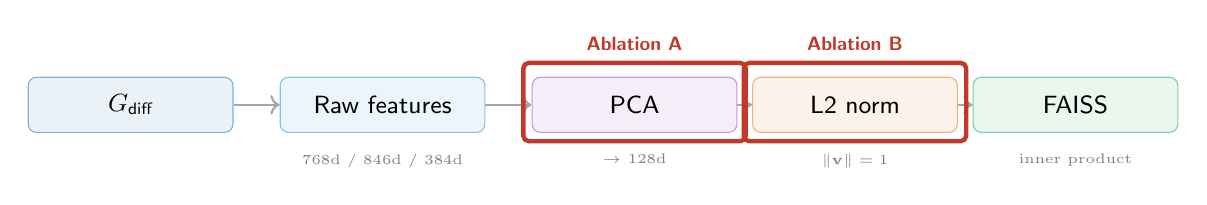
\begin{tikzpicture}[
    box/.style={rounded corners=3pt, draw=#1!60, fill=#1!10,
                minimum width=2.6cm, minimum height=0.7cm,
                font=\small\sffamily, align=center},
    arr/.style={->, thick, gray!70},
    ablbl/.style={font=\scriptsize\sffamily\bfseries, #1}]

    % pipeline boxes
    \node[box=c1]  (graph)  at (0,0)     {$G_{\text{diff}}$};
    \node[box=c2]  (feat)   at (3.2,0)   {Raw features};
    \node[box=c3]  (pca)    at (6.4,0)   {PCA};
    \node[box=c5]  (l2)     at (9.2,0)   {L2 norm};
    \node[box=hit] (faiss)  at (12.0,0)  {FAISS};

    \draw[arr] (graph) -- (feat);
    \draw[arr] (feat)  -- (pca);
    \draw[arr] (pca)   -- (l2);
    \draw[arr] (l2)    -- (faiss);

    % dimension annotations
    \node[below=4pt, font=\tiny\color{black!50}] at (feat.south) {768d / 846d / 384d};
    \node[below=4pt, font=\tiny\color{black!50}] at (pca.south) {$\to$ 128d};
    \node[below=4pt, font=\tiny\color{black!50}] at (l2.south) {$\|\mathbf{v}\|=1$};
    \node[below=4pt, font=\tiny\color{black!50}] at (faiss.south) {inner product};

    % ablation markers
    \draw[miss, ultra thick, rounded corners=2pt]
      ([shift={(-3pt,5pt)}]pca.north west) rectangle ([shift={(3pt,-3pt)}]pca.south east);
    \node[ablbl=miss, above=6pt] at (pca.north) {Ablation A};

    \draw[miss, ultra thick, rounded corners=2pt]
      ([shift={(-3pt,5pt)}]l2.north west) rectangle ([shift={(3pt,-3pt)}]l2.south east);
    \node[ablbl=miss, above=6pt] at (l2.north) {Ablation B};
  \end{tikzpicture}

  \vspace{0.8em}
  \begin{columns}[T]
  \begin{column}{0.48\textwidth}
    \textbf{PCA} {\small(dimensionality reduction)}
    \begin{itemize}\setlength{\itemsep}{2pt}
      {\scriptsize
      \item Projects high-dim features to 128d
      \item Learns optimal linear basis from data
      \item Decorrelates and compresses — fuses heterogeneous streams (e.g.\ 78d structural $+$ 768d CodeBERT)}
    \end{itemize}
  \end{column}
  \begin{column}{0.48\textwidth}
    \textbf{L2 normalization} {\small(scale invariance)}
    \begin{itemize}\setlength{\itemsep}{2pt}
      {\scriptsize
      \item Maps every embedding onto the unit hypersphere
      \item FAISS inner product $=$ cosine similarity
      \item Similarity depends on \textbf{direction} (pattern), not \textbf{magnitude} (graph size)}
    \end{itemize}
  \end{column}
  \end{columns}
\end{frame}


\begin{frame}{Ablation Results: PCA and L2 Normalization ($n{=}225$, self-retrieval)}

  \centering
  \vspace{0.2em}
  {\small
  \renewcommand{\arraystretch}{1.35}
  \setlength{\tabcolsep}{5pt}
  \begin{tabular}{l *{3}{c} c *{3}{c} c *{3}{c}}
    \toprule
    & \multicolumn{3}{c}{\textbf{PCA + L2} {\footnotesize(baseline)}}
    && \multicolumn{3}{c}{\textbf{No PCA, L2 only} {\footnotesize(Abl.\ A)}}
    && \multicolumn{3}{c}{\textbf{No PCA, no L2} {\footnotesize(Abl.\ B)}} \\
    \cmidrule{2-4} \cmidrule{6-8} \cmidrule{10-12}
    \textbf{Embedder}
      & hit@1 & MRR & CWE
      && hit@1 & MRR & CWE
      && hit@1 & MRR & CWE \\
    \midrule
    \rowcolor{c1!12}
    Combined
      & \chit{84.9\%} & \chit{.890} & \chit{.501}
      && \cwarn{74.0\%} & .780 & .398
      && \cmiss{1.4\%} & .047 & .071 \\
    CodeBERT seq
      & 75.3\% & .793 & .412
      && 76.7\% & .799 & .402
      && \cmiss{1.4\%} & .107 & .160 \\
    GIN
      & 72.6\% & .788 & .443
      && 72.6\% & .788 & .443
      && \cmiss{1.4\%} & .044 & .068 \\
    CodeBERT pat.
      & 71.2\% & .768 & .414
      && 75.3\% & .788 & .394
      && \cmiss{1.4\%} & .132 & .201 \\
    WL
      & 65.8\% & .720 & .423
      && 67.1\% & .723 & .435
      && \cmiss{0.0\%} & .045 & .065 \\
    RGCN
      & 60.3\% & .676 & .372
      && \cwarn{67.1\%} & .733 & .390
      && \cmiss{0.0\%} & .014 & .060 \\
    \bottomrule
  \end{tabular}}

  \vspace{0.6em}
  \begin{columns}[T]
  \begin{column}{0.32\textwidth}
    {\small\textbf{\textcolor{hit}{Baseline: PCA + L2}}}
    \begin{itemize}\setlength{\itemsep}{2pt}
      {\scriptsize
      \item Combined dominates: 84.9\%
      \item PCA is critical for Combined ($-$10.9~pp without)}
    \end{itemize}
  \end{column}
  \begin{column}{0.32\textwidth}
    {\small\textbf{\textcolor{warn}{Abl.\ A: No PCA}}}
    \begin{itemize}\setlength{\itemsep}{2pt}
      {\scriptsize
      \item CodeBERT stable ($\pm$1~pp)
      \item GIN identical — already 128d
      \item Combined collapses: PCA fuses the 3 sub-embedders}
    \end{itemize}
  \end{column}
  \begin{column}{0.32\textwidth}
    {\small\textbf{\textcolor{miss}{Abl.\ B: No L2}}}
    \begin{itemize}\setlength{\itemsep}{2pt}
      {\scriptsize
      \item \textbf{Catastrophic failure} — all $<$2\%
      \item Mean sim $>$100k (magnitude dominates)
      \item L2 norm is non-negotiable}
    \end{itemize}
  \end{column}
  \end{columns}
\end{frame}

% ══════════════════════════════════════════════════════════════════════
\section{Embedding Pipeline Ablation}
% ══════════════════════════════════════════════════════════════════════


\begin{frame}{Embedding Space Analysis: Metrics}
\begin{columns}[T]
\begin{column}{0.48\textwidth}

  \textbf{\textcolor{c1}{Single-space quality}} {\small(per embedder)}

  \vspace{0.3em}
  {\scriptsize
  \renewcommand{\arraystretch}{1.25}
  \begin{tabular}{p{2.0cm}p{4.8cm}}
    \toprule
    \textbf{Metric} & \textbf{What it measures} \\
    \midrule
    Isotropy
      & Are embeddings spread uniformly across directions?
        Low $\to$ a few dimensions dominate $\to$ retrieval degrades. \\
    Hubness
      & Do some points appear as neighbors of \emph{everyone}?
        High skewness $\to$ false-positive retrievals. \\
    Alignment / Uniformity
      & \textbf{Alignment}: same-CWE pairs are close.
        \textbf{Uniformity}: all points spread on hypersphere.
        Decomposes retrieval quality into two axes. \\
    Intra/Inter ratio
      & $\frac{\text{mean intra-CWE sim}}{\text{mean inter-CWE sim}}$.
        $>$1 means classes separated $\to$ good CWE recall. \\
    Distance concentration
      & $\frac{d_{\max} - d_{\min}}{d_{\min}}$ per query.
        Low $\to$ all distances alike $\to$ cosine unreliable. \\
    \bottomrule
  \end{tabular}}

\end{column}
\begin{column}{0.48\textwidth}

  \textbf{\textcolor{c3}{Cross-space comparison}} {\small(Combined vs.\ individual)}

  \vspace{0.3em}
  {\scriptsize
  \renewcommand{\arraystretch}{1.25}
  \begin{tabular}{p{2.2cm}p{4.6cm}}
    \toprule
    \textbf{Metric} & \textbf{What it measures} \\
    \midrule
    Linear CKA
      & Structural similarity between two embedding matrices.
        Invariant to rotation/scaling.
        High $\to$ spaces encode the same geometry. \\
    $k$-NN overlap
      & \% shared neighbors between two spaces.
        High $\to$ same retrieval behavior (redundant).
        Low $\to$ complementary signal. \\
    Rank correlation
      & Spearman $\rho$ of pairwise distances.
        High $\to$ one embedder dominates the fusion. \\
    Trustworthiness
      & Did PCA (384d$\to$128d) distort local neighborhoods?
        1.0 $=$ perfect preservation.
        Low $\to$ PCA causes retrieval errors. \\
    \bottomrule
  \end{tabular}}

  \vspace{0.5em}
  {\scriptsize\textcolor{c1}{\faIcon{bullseye}}
  \textbf{Why these metrics?}}

  \vspace{0.2em}
  {\scriptsize
  \begin{itemize}\setlength{\itemsep}{1pt}
    \item Diagnose \emph{why} Combined outperforms individuals
    \item Identify which sub-embedder dominates the PCA
    \item Detect degenerate spaces \emph{before} running retrieval
    \item Explain per-query errors via space properties
  \end{itemize}}

\end{column}
\end{columns}
\end{frame}

\begin{frame}{Embedding Space Analysis: Experiment Design}
\begin{columns}[T]
\begin{column}{0.50\textwidth}

  \textbf{Setup} {\small(same split as retrieval experiments)}

  \vspace{0.3em}
  {\scriptsize
  \begin{itemize}\setlength{\itemsep}{3pt}
    \item 225 index graphs ($G_{\text{diff}}$), seed$=$42, stratified
    \item 6 embedders: Combined, GIN, WL, CodeBERT seq, CodeBERT pat., RGCN
    \item All projected to 128d (PCA) $+$ L2-normalized
    \item CWE labels as class signal ($\sim$15 unique classes)
  \end{itemize}}

  \vspace{0.5em}
  \textbf{Analysis structure} {\small(no grid — fixed dataset)}

  \vspace{0.3em}
  {\scriptsize
  \renewcommand{\arraystretch}{1.25}
  \begin{tabular}{p{2.2cm}p{4.8cm}}
    \toprule
    \textbf{Analysis} & \textbf{Output} \\
    \midrule
    Per-embedder
      & Isotropy, hubness, alignment/uniformity, intra/inter,
        distance concentration \\
    Pairwise matrices
      & $6 \times 6$ CKA, $k$-NN overlap, rank correlation \\
    Combined PCA
      & Trustworthiness at $k \in \{5, 10, 20\}$ \\
    Sensitivity
      & Hubness skewness vs.\ $k$ (stability check) \\
    \bottomrule
  \end{tabular}}

\end{column}
\begin{column}{0.47\textwidth}

  \textbf{Key questions this answers}

  \vspace{0.3em}
  {\scriptsize
  \begin{enumerate}\setlength{\itemsep}{4pt}
    \item \textbf{Does Combined add value?}\\
      If CKA(Combined, GIN) $\approx 1$ $\to$ Combined $\approx$ GIN with extra cost.\\
      If $k$-NN overlap is low $\to$ Combined retrieves differently.

    \item \textbf{Which sub-embedder dominates?}\\
      Rank correlation identifies whose distance structure is preserved in the fusion.

    \item \textbf{Is PCA lossy?}\\
      Trustworthiness $< 0.9$ $\to$ PCA distorts neighborhoods $\to$ explains Combined-specific misses.

    \item \textbf{Why do some CWEs fail?}\\
      Per-CWE intra/inter ratio shows which classes overlap in each space.

    \item \textbf{Are there hub points?}\\
      Hub fraction $> 5\%$ $\to$ some samples ``attract'' queries $\to$ systematic false positives.
  \end{enumerate}}

  \vspace{0.4em}
  {\scriptsize\color{black!55}
  Run: \texttt{python -m experiments.space\_analysis\_experiment}}

\end{column}
\end{columns}
\end{frame}


% ══════════════════════════════════════════════════════════════════════
\section{Embedding Combination Strategies}
% ══════════════════════════════════════════════════════════════════════

\begin{frame}[fragile]{Combination Strategies: Experiment Design}
\begin{columns}[T]
\begin{column}{0.50\textwidth}

  \textbf{Goal}\\[3pt]
  {\small The Combined embedder concatenates NetLSD~$+$~WL~$+$~GIN
  then reduces with PCA\@.  Does pre-processing each sub-embedder
  \emph{before} concatenation improve the fused space?}

  \vspace{0.6em}
  \textbf{Strategies compared}

  \vspace{0.2em}
  {\scriptsize
  \renewcommand{\arraystretch}{1.25}
  \begin{tabular}{p{2.2cm}p{4.8cm}}
    \toprule
    \textbf{Strategy} & \textbf{Pipeline} \\
    \midrule
    \texttt{concat\_pca}
      & Concatenate raw $\to$ PCA to 128d {\small(baseline)} \\
    \texttt{pca\_concat\_pca}
      & PCA each to 128d $\to$ concat (384d) $\to$ PCA to 128d \\
    \texttt{pca\_concat}
      & PCA each to 42d $\to$ concat to 126d {\small(no 2\textsuperscript{nd} PCA)} \\
    \texttt{norm\_concat\_pca}
      & L2-norm each $\to$ concat $\to$ PCA to 128d \\
    \bottomrule
  \end{tabular}}

  \vspace{0.4em}
  \textbf{Rationale}\\[2pt]
  {\scriptsize Individual PCA or normalization could equalize sub-embedder
  scales and remove noise before fusion.  Alternatively, a single
  final PCA may better exploit cross-embedder correlations.}

\end{column}
\begin{column}{0.47\textwidth}

  \centering
  \vspace{0.5em}
  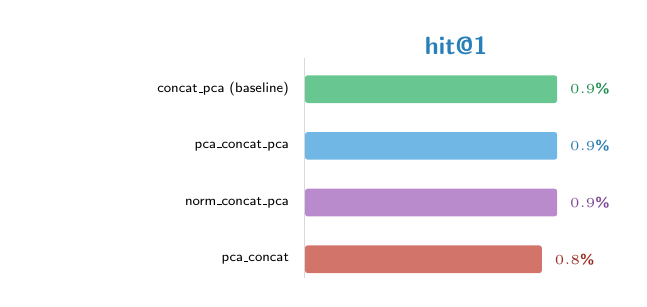
\begin{tikzpicture}[scale=0.8]
    \foreach \y/\lbl/\col/\val in {
      2.7/{concat\_pca (baseline)}/hit/0.890,
      1.8/{pca\_concat\_pca}/c2/0.890,
      0.9/{norm\_concat\_pca}/c3/0.890,
      0.0/{pca\_concat}/miss/0.836}{
      \node[left,font=\tiny\sffamily,text width=3.2cm,align=right] at (0,\y) {\lbl};
      \fill[\col!70,rounded corners=1pt] (0.1,\y-0.22) rectangle ({0.1+4.5*\val},\y+0.22);
      \node[right,font=\tiny\sffamily\bfseries,\col!80!black] at ({0.1+4.5*\val+0.05},\y)
        {\pgfmathprintnumber[fixed,precision=1]{\val}\%};
    }
    \draw[black!15] (0.1,-0.3)--(0.1,3.2);
    \node[above,font=\small\sffamily\bfseries,c1] at (2.5,3.1) {hit@1};
  \end{tikzpicture}

  \vspace{0.6em}
  {\scriptsize\color{black!55}
  225 index, 73 query ($G_{\text{diff}}$, seed$=$42).\\
  Each sub-embedder: 128d (NetLSD, WL, GIN).\\
  Run: \texttt{python -m experiments.combining\_experiment}}

\end{column}
\end{columns}
\end{frame}


\begin{frame}{Combination Strategies: Results ($n{=}73$)}

  \centering
  \vspace{0.2em}
  {\small
  \renewcommand{\arraystretch}{1.35}
  \setlength{\tabcolsep}{4.5pt}
  \begin{tabular}{l *{6}{c} c *{4}{c}}
    \toprule
    & \multicolumn{6}{c}{\textbf{Retrieval}}
    && \multicolumn{4}{c}{\textbf{Space Quality}} \\
    \cmidrule{2-7} \cmidrule{9-12}
    \textbf{Strategy}
      & hit@1 & hit@5 & hit@10 & MRR & nDCG@10 & MAP@10
      && Eff.\ Dim & Isotropy & Hub Skew & Intra/Inter \\
    \midrule
    \rowcolor{c1!12}
    \texttt{concat\_pca}
      & \chit{89.0\%} & 95.9\% & 97.3\% & \chit{.915} & \chit{.687} & \chit{.567}
      && \chit{30.9} & .0024 & 1.40 & \chit{2.07} \\
    \texttt{pca\_concat\_pca}
      & \chit{89.0\%} & 95.9\% & 97.3\% & \chit{.915} & \chit{.687} & \chit{.567}
      && \chit{30.9} & .0023 & 1.40 & \chit{2.07} \\
    \texttt{norm\_concat\_pca}
      & \chit{89.0\%} & 95.9\% & 97.3\% & \chit{.915} & \chit{.687} & \chit{.567}
      && \chit{30.9} & .0024 & 1.40 & \chit{2.07} \\
    \texttt{pca\_concat}
      & \cmiss{83.6\%} & 95.9\% & 97.3\% & \cwarn{.882} & \cwarn{.665} & \cwarn{.538}
      && \cwarn{23.0} & \cmiss{$\approx$0} & 1.09 & \cwarn{1.87} \\
    \bottomrule
  \end{tabular}}

  \vspace{0.5em}
  \begin{columns}[T]
  \begin{column}{0.32\textwidth}
    {\small\textbf{\textcolor{hit}{Baseline is optimal}}}
    \begin{itemize}\setlength{\itemsep}{2pt}
      {\scriptsize
      \item Three strategies are \textbf{identical} to 4+ decimal places
      \item Sub-embedders already output 128d L2-normed vectors $\to$ pre-processing is a no-op}
    \end{itemize}
  \end{column}
  \begin{column}{0.32\textwidth}
    {\small\textbf{\textcolor{miss}{\texttt{pca\_concat} hurts}}}
    \begin{itemize}\setlength{\itemsep}{2pt}
      {\scriptsize
      \item hit@1 drops $-$5.4~pp, MRR $-$3.3~pp
      \item PCA to 42d per embedder loses too much information
      \item Isotropy collapses ($\approx$0): space degenerate}
    \end{itemize}
  \end{column}
  \begin{column}{0.32\textwidth}
    {\small\textbf{\textcolor{c1}{Why single PCA wins}}}
    \begin{itemize}\setlength{\itemsep}{2pt}
      {\scriptsize
      \item Final PCA over full 384d can exploit \textbf{cross-embedder correlations}
      \item Independent per-embedder PCA cannot discover joint structure
      \item Eff.\ dim 30.9 vs.\ 23.0: richer space}
    \end{itemize}
  \end{column}
  \end{columns}
\end{frame}


\begin{frame}{Combination Strategies: Key Findings}

  \begin{enumerate}\setlength{\itemsep}{0.5em}

    \item[\textcolor{hit}{\faIcon{check-circle}}]
      \textbf{Current pipeline is already well-conditioned.}
      Pre-normalizing or pre-reducing individual embeddings before concatenation
      adds zero measurable benefit --- the sub-embedders already produce
      128d L2-normalized vectors.
      \textit{No pipeline change needed.}

    \vspace{0.5em}
    \item[\textcolor{miss}{\faIcon{compress-arrows-alt}}]
      \textbf{Double PCA without final reduction = information loss.}
      Reducing each embedder to 42d then concatenating (126d, no second PCA)
      drops hit@1 by 5.4~pp and collapses isotropy to $\approx$0.
      \textit{The final PCA is essential --- it finds the best 128 directions across
      the full 384d concatenated space.}

    \vspace{0.5em}
    \item[\textcolor{c1}{\faIcon{chart-bar}}]
      \textbf{Cross-embedder correlations matter.}
      A single PCA over the joint space (eff.\ dim 30.9) outperforms
      three independent PCAs (eff.\ dim 23.0) because it captures
      shared structure between NetLSD, WL, and GIN\@.

    \vspace{0.5em}
    \item[\textcolor{c3}{\faIcon{lightbulb}}]
      \textbf{Implication for future embedders.}
      When adding new sub-embedders (e.g.\ CodeBERT), they shou
% Integrating codebert into the Combined embedder is a promising future direction, but requires careful tuning to ensure the fused space remains well-conditioned for retrieval.  Our current analysis suggests that the existing PCA + L2 normalization pipeline is robust to adding new sub-embedders without modification, but empirical validation with CodeBERT is needed.
ld be
      concatenated raw into the joint space and let PCA handle fusion ---
      no per-embedder preprocessing is warranted.

  \end{enumerate}
\end{frame}

% Integrating codebert into the Combined embedder is a promising future direction, but requires careful tuning to ensure the fused space remains well-conditioned for retrieval.  Our current analysis suggests that the existing PCA + L2 normalization pipeline is robust to adding new sub-embedders without modification, but empirical validation with CodeBERT is needed.


% ══════════════════════════════════════════════════════════════════════
\section{4-Way Fusion: Adding CodeBERT-Pattern}
% ══════════════════════════════════════════════════════════════════════

\begin{frame}[fragile]{4-Way Fusion: Experiment Design}
\begin{columns}[T]
\begin{column}{0.50\textwidth}

  \textbf{Goal}\\[3pt]
  {\small Can adding a semantic signal (CodeBERT-pattern) to the structural
  fusion (NetLSD~$+$~WL~$+$~GIN) improve retrieval?
  We test two hypotheses:
  (1)~raw concat lets PCA discover joint directions,
  (2)~pre-PCA'ing CodeBERT to 128d equalises scale.}

  \vspace{0.5em}
  \textbf{Run 1: raw concatenation}\\[2pt]
  {\scriptsize CodeBERT-pattern emits 802d (34 pattern $+$ 768 CodeBERT).
  Concat with 3$\times$128d structural $=$ 1186d $\to$ PCA to 128d.\\
  \textbf{Problem:} CodeBERT contributes 68\% of dimensions.}

  \vspace{0.5em}
  \textbf{Run 2: balanced pre-PCA}\\[2pt]
  {\scriptsize PCA CodeBERT-pattern 802d~$\to$~128d first,
  then concat 4$\times$128d $=$ 512d $\to$ PCA to 128d.\\
  Each sub-embedder gets 25\% of the pre-PCA space.}

  \vspace{0.5em}
  \textbf{Rationale}\\[3pt]
  {\small CodeBERT captures code \textit{semantics}; structural embedders
  capture vulnerability \textit{patterns}. Low CKA between them
  in prior experiments suggests complementary signals.}

\end{column}
\begin{column}{0.47\textwidth}

  \centering
  \vspace{0.3em}
  {\small\textbf{Pipeline comparison}}

  \vspace{0.3em}
  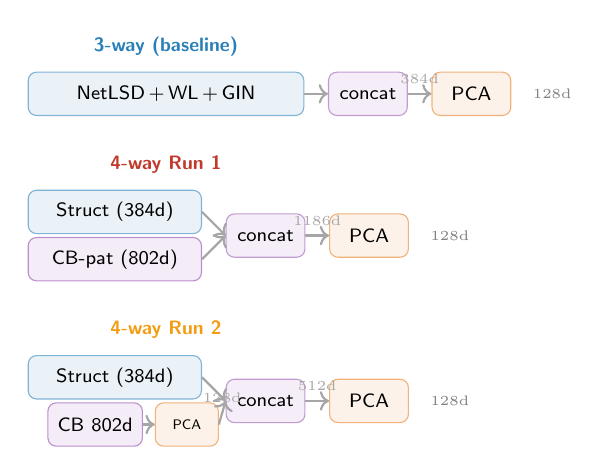
\begin{tikzpicture}[
    box/.style={rounded corners=3pt, draw=#1!60, fill=#1!10,
                minimum height=0.55cm, font=\scriptsize\sffamily, align=center},
    arr/.style={->, thick, gray!70},
    node distance=0.3cm]

    % 3-way baseline
    \node[font=\scriptsize\sffamily\bfseries,c1] (lbl3) at (0,2.3) {3-way (baseline)};
    \node[box=c1, minimum width=3.5cm] (c3) at (0,1.7) {NetLSD\,+\,WL\,+\,GIN};
    \node[box=c3, right=0.3cm of c3, minimum width=1cm] (cat3) {concat};
    \node[box=c5, right=0.3cm of cat3, minimum width=1cm] (pca3) {PCA};
    \draw[arr] (c3) -- (cat3);
    \draw[arr] (cat3) -- node[above,font=\tiny] {384d} (pca3);
    \node[right=0.15cm of pca3, font=\tiny\color{black!50}] {128d};

    % 4-way run 1
    \node[font=\scriptsize\sffamily\bfseries,miss] (lbl4a) at (0,0.8) {4-way Run 1};
    \node[box=c1, minimum width=2.2cm] (s4a) at (-0.65,0.2) {Struct (384d)};
    \node[box=c4, minimum width=2.2cm] (cb4a) at (-0.65,-0.4) {CB-pat (802d)};
    \node[box=c3, right=0.3cm of s4a, minimum width=1cm, yshift=-0.3cm] (cat4a) {concat};
    \node[box=c5, right=0.3cm of cat4a, minimum width=1cm] (pca4a) {PCA};
    \draw[arr] (s4a.east) -- (cat4a.west);
    \draw[arr] (cb4a.east) -- (cat4a.west);
    \draw[arr] (cat4a) -- node[above,font=\tiny] {1186d} (pca4a);
    \node[right=0.15cm of pca4a, font=\tiny\color{black!50}] {128d};

    % 4-way run 2
    \node[font=\scriptsize\sffamily\bfseries,warn] (lbl4b) at (0,-1.3) {4-way Run 2};
    \node[box=c1, minimum width=2.2cm] (s4b) at (-0.65,-1.9) {Struct (384d)};
    \node[box=c4, minimum width=1.2cm] (cb4b) at (-0.9,-2.5) {CB 802d};
    \node[box=c5, right=0.15cm of cb4b, minimum width=0.8cm] (pcb) {\tiny PCA};
    \node[box=c3, right=0.3cm of s4b, minimum width=1cm, yshift=-0.3cm] (cat4b) {concat};
    \node[box=c5, right=0.3cm of cat4b, minimum width=1cm] (pca4b) {PCA};
    \draw[arr] (s4b.east) -- (cat4b.west);
    \draw[arr] (cb4b) -- (pcb);
    \draw[arr] (pcb.east) -- node[above,font=\tiny] {128d} (cat4b.west);
    \draw[arr] (cat4b) -- node[above,font=\tiny] {512d} (pca4b);
    \node[right=0.15cm of pca4b, font=\tiny\color{black!50}] {128d};
  \end{tikzpicture}

\end{column}
\end{columns}
\end{frame}


\begin{frame}{4-Way Fusion: Results}

  \centering
  \vspace{0.1em}
  {\small
  \renewcommand{\arraystretch}{1.35}
  \setlength{\tabcolsep}{3.5pt}
  \begin{tabular}{l *{4}{c} c *{4}{c}}
    \toprule
    & \multicolumn{4}{c}{\textbf{Retrieval}}
    && \multicolumn{4}{c}{\textbf{Space Quality}} \\
    \cmidrule{2-5} \cmidrule{7-10}
    \textbf{Strategy}
      & hit@1 & hit@5 & MRR & nDCG@10
      && Eff.\ Dim & Isotropy & Mean Sim & Intra/Inter \\
    \midrule
    \rowcolor{c1!12}
    3-way baseline
      & \chit{90.4\%} & \chit{95.9\%} & \chit{.928} & \chit{.690}
      && \chit{31.2} & .0023 & .030 & \chit{2.30} \\
    \addlinespace[2pt]
    4-way raw concat
      & \cmiss{74.0\%} & \cmiss{86.3\%} & \cmiss{.786} & \cmiss{.572}
      && \cwarn{19.3} & .0029 & \cmiss{$-$.004} & \cmiss{$-$6.46} \\
    {\scriptsize (Run~1: 1186d$\to$128d)}
      & & & & && & & & \\
    \addlinespace[2pt]
    4-way pre-PCA
      & \cmiss{74.0\%} & \cmiss{86.3\%} & \cmiss{.786} & \cmiss{.572}
      && \cwarn{19.2} & .0028 & \cmiss{$-$.004} & \cmiss{$-$6.59} \\
    {\scriptsize (Run~2: 512d$\to$128d)}
      & & & & && & & & \\
    \bottomrule
  \end{tabular}}

  \vspace{0.5em}
  \begin{columns}[T]
  \begin{column}{0.32\textwidth}
    {\small\textbf{\textcolor{miss}{CodeBERT hurts: $-$16~pp}}}
    \begin{itemize}\setlength{\itemsep}{2pt}
      {\scriptsize
      \item hit@1 drops from 90.4\% to 74.0\%
      \item MRR drops from .928 to .786
      \item Both runs produce \textbf{identical} degradation}
    \end{itemize}
  \end{column}
  \begin{column}{0.32\textwidth}
    {\small\textbf{\textcolor{warn}{Pre-PCA doesn't help}}}
    \begin{itemize}\setlength{\itemsep}{2pt}
      {\scriptsize
      \item Equalising dimensions (512d) gives same result as raw (1186d)
      \item Problem is \textbf{signal conflict}, not scale imbalance
      \item CodeBERT dominates PCA regardless}
    \end{itemize}
  \end{column}
  \begin{column}{0.32\textwidth}
    {\small\textbf{\textcolor{c1}{Space explains the failure}}}
    \begin{itemize}\setlength{\itemsep}{2pt}
      {\scriptsize
      \item \textbf{Negative mean sim} ($-$0.004): embeddings anti-correlated
      \item \textbf{Negative intra/inter} ($-$6.5): class structure inverted
      \item Eff.\ dim 19 vs.\ 31: PCA captures wrong directions}
    \end{itemize}
  \end{column}
  \end{columns}
\end{frame}


\begin{frame}{4-Way Fusion: Key Findings}

  \begin{enumerate}\setlength{\itemsep}{0.5em}

    \item[\textcolor{miss}{\faIcon{times-circle}}]
      \textbf{CodeBERT-pattern is incompatible with structural fusion.}
      Adding it degrades every metric by 15--16~pp.
      The semantic signal encodes \textit{what code does}, not
      \textit{how the vulnerability manifests structurally} ---
      these are contradictory for CWE discrimination.
      \textit{The signals destructively interfere in PCA.}

    \vspace{0.5em}
    \item[\textcolor{warn}{\faIcon{balance-scale}}]
      \textbf{Dimension balancing is not the fix.}
      Pre-PCA'ing CodeBERT to 128d (equal to each structural embedder)
      produces identical results to raw 802d concatenation.
      PCA's top components still reflect CodeBERT's high-variance
      semantic directions, not vulnerability-discriminative structure.

    \vspace{0.5em}
    \item[\textcolor{c1}{\faIcon{chart-bar}}]
      \textbf{Negative intra/inter ratio is the diagnostic.}
      Same-CWE pairs become \textit{less} similar than cross-CWE pairs
      ($-$6.5 ratio). Two functions with the same CWE can have very
      different code semantics --- CodeBERT sees them as ``different''
      and overrides the structural ``same-pattern'' signal.

    \vspace{0.5em}
    \item[\textcolor{c3}{\faIcon{lightbulb}}]
      \textbf{If CodeBERT is to help, it needs late fusion.}
      Concatenation + PCA is early fusion and fails here.
      Alternatives: separate retrieval pipelines with score-level
      combination (RRF), learned gating, or reranking with CodeBERT
      as a second stage.

  \end{enumerate}
\end{frame}


% ══════════════════════════════════════════════════════════════════════
\section{Agent Baseline}
% ══════════════════════════════════════════════════════════════════════

\begin{frame}{Agent Baseline: Experiment Design}
\begin{columns}[T]
\begin{column}{0.52\textwidth}

  \textbf{Goal}\\[3pt]
  {\small Given a vulnerable function and a retrieved similar CVE,
  can an LLM generate a correct patch \textbf{by analogy}?
  Compare \textit{oracle} retrieval (perfect) vs.\ \textit{embedding} retrieval (our pipeline).}

  \vspace{0.6em}
  \textbf{Model \& prompt}
  \begin{itemize}\setlength{\itemsep}{2pt}
    {\scriptsize
    \item \textbf{GPT-4o} (Azure), temperature$=$0.2, max\_tokens$=$4096
    \item \textbf{One-shot patching by analogy}: system prompt contains the
          retrieved CVE's fix-list, variable/function mapping, root cause
    \item Assistant message shows the example's CoT + patched code
    \item User message provides the target function to patch
    \item Agent must output \texttt{[CoT START]...[Patched Code END]}}
  \end{itemize}

\end{column}
\begin{column}{0.45\textwidth}

  \textbf{Retrieval modes}

  \vspace{0.3em}
  {\small
  \renewcommand{\arraystretch}{1.25}
  \begin{tabular}{p{1.5cm}p{4.5cm}}
    \toprule
    \textbf{Mode} & \textbf{What it retrieves} \\
    \midrule
    \textbf{Oracle}
      & Same-CVE pair from index (perfect match) — upper bound on agent quality \\
    \textbf{Embedding}
      & Top-1 from Combined embedder + FAISS (realistic pipeline) \\
    \bottomrule
  \end{tabular}}

  \vspace{0.5em}
  \textbf{Evaluation protocol}
  \begin{itemize}\setlength{\itemsep}{2pt}
    {\scriptsize
    \item Same split: 225 index, 73 query (seed$=$42)
    \item \textbf{Patch quality}: BLEU-4, token Jaccard, CodeBLEU proxy
    \item \textbf{Retrieval}: hit@1, MRR, CWE hit@5
    \item \textbf{Confidence}: precision/recall at score thresholds}
  \end{itemize}

\end{column}
\end{columns}
\end{frame}



\begin{frame}{Agent Baseline: Analysis \& Failure Modes}
\begin{columns}[T]
\begin{column}{0.50\textwidth}

  \textbf{Where the agent succeeds}
 

  \vspace{0.5em}
  \textbf{Where the agent fails}


\end{column}
\begin{column}{0.47\textwidth}

  \textbf{Oracle vs.\ Embedding: what the gap tells us}

  \vspace{0.3em}
  \begin{itemize}\setlength{\itemsep}{3pt}
    {\scriptsize
    \item Patch quality \textbf{degrades with retrieval accuracy}:
          CBP .557 (oracle) vs.\ .409 (embedding), $-$15~pp
    \item When retrieval misses the correct CVE (31.5\% of queries),
          the analogy is less relevant $\to$ lower patch quality
    \item Both retrieval \textbf{and} generation quality are bottlenecks}
  \end{itemize}

  \vspace{0.5em}
  \textbf{Open questions for improvement}
  \begin{itemize}\setlength{\itemsep}{3pt}
    {\scriptsize
    \item Future work on hybrid retrieval approaches
    \item Cross-validation with other CVE datasets}
  \end{itemize}


\end{column}
\end{columns}
\end{frame}

\begin{frame}[plain]
\centering
\vspace{3em}
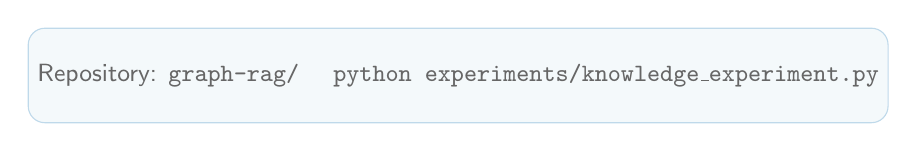
\begin{tikzpicture}
  \node[draw=c1!30,rounded corners=6pt,fill=c1!5,
        minimum width=9cm,minimum height=1.2cm,
        font=\small\sffamily\color{black!60},align=center]
    {Repository: \texttt{graph-rag/} \quad
     \texttt{python experiments/knowledge\_experiment.py}};
\end{tikzpicture}
\end{frame}

\end{document}
